% Created 2020-05-15 Fri 16:57
% Intended LaTeX compiler: pdflatex
\documentclass[11pt]{article}
\usepackage[utf8]{inputenc}
\usepackage[T1]{fontenc}
\usepackage{graphicx}
\usepackage{grffile}
\usepackage{longtable}
\usepackage{wrapfig}
\usepackage{rotating}
\usepackage[normalem]{ulem}
\usepackage{amsmath}
\usepackage{textcomp}
\usepackage{amssymb}
\usepackage{capt-of}
\usepackage{hyperref}
\usepackage{minted}
\usepackage[a4paper,margin=20mm]{geometry}
\usepackage{amsmath}
\usepackage{amsfonts}
\usepackage{stmaryrd}
\usepackage{bm}
\usepackage{sidecap}
\usepackage{minted}
\usemintedstyle{emacs}
\usepackage[T1]{fontenc}
\usepackage[scaled]{beraserif}
\usepackage[scaled]{berasans}
\usepackage[scaled]{beramono}
\newcommand{\tr}{\textsf{T}}
\newcommand{\grad}{\bm{\nabla}}
\newcommand{\av}[2][]{\mathbb{E}_{#1\!}\left[ #2 \right]}
\newcommand{\Prob}[2][]{\mathbb{P}_{#1\!}\left[ #2 \right]}
\newcommand{\logg}[1]{\log\!\left( #1 \right)}
\newcommand{\pred}[1]{\left\llbracket { \small #1} \right\rrbracket}
\newcommand{\e}[1]{{\rm e}^{#1}}
\newcommand{\dd}{\mathrm{d}}
\newcommand{\ii}{\mathrm{i}}
\DeclareMathAlphabet{\mat}{OT1}{cmss}{bx}{n}
\newcommand{\normal}[2]{\mathcal{N}\!\left(#1 \big| #2 \right)}
\newcounter{eqCounter}
\setcounter{eqCounter}{0}
\newcommand{\explanation}{\setcounter{eqCounter}{0}\renewcommand{\labelenumi}{(\arabic{enumi})}}
\newcommand{\eq}[1][=]{\stepcounter{eqCounter}\stackrel{\text{\tiny(\arabic{eqCounter})}}{#1}}
\newcommand{\argmax}{\mathop{\mathrm{argmax}}}
\newcommand{\Dist}[2][Binom]{\mathrm{#1}\left( \strut {#2} \right)}
\newcommand{\RNA}{\mathit{RNA}}
\author{Adam Prügel-Bennett}
\date{\today}
\title{Computational Biology Subsidary Notes\\\medskip
\large Lecture 16: Gene Regulation Networks}
\hypersetup{
 pdfauthor={Adam Prügel-Bennett},
 pdftitle={Computational Biology Subsidary Notes},
 pdfkeywords={},
 pdfsubject={},
 pdfcreator={Emacs 26.3 (Org mode 9.1.9)}, 
 pdflang={English}}
\begin{document}

\maketitle

\section{Keywords}
\label{sec:org82530e7}
\begin{itemize}
\item Evolution, DNA, Proteins
\end{itemize}

\section{Main Points}
\label{sec:org8cab513}

\subsection{Gene Regulation Networks}
\label{sec:org61f900e}
\begin{itemize}
\item We are currently in a phase of science where we are beginning to
understand how cells regulate themselves
\item A major mechanism is through switching on and off the expression
of proteins
\item This happens through \emph{transcription factors} (proteins) which
\begin{itemize}
\item sensing the environment (often through signalling molecules)
\item bind to the promoter regions of DNA
\item excite or inhibit the transcription of RNA for the
corresponding protein
\end{itemize}
\item There is a complex networks of interactions making it very
challenging to understand what is going on
\end{itemize}

q** Chemical Equations
\begin{itemize}
\item The gene regulation process is a dynamic process
\item Reactions happen on different time scales
\begin{itemize}
\item This helps us: we are usually interested in what happens on the slow
time scale
\item Fast reactions can be assumed to reach their equilibrium state instantaneously
\item Proteins binding with small (signalling) molecules will happen
in milliseconds
\item A transcription factor protein will bind with the promoter
region in a few second
\item The transcription and translation of a gene to a protein takes
around 5 minutes
\item The change in the concentration of a protein by 50\% takes about
an hour
\end{itemize}
\item To model the dynamics we start from "\emph{chemical equations}"
\begin{itemize}
\item These are not what chemists would recognise as chemical equations
\item They don't respect conservation of matter
\item This is because they only capture the slow processes and ignore
fast processes (the equations would be far too complicated to
be useful if they described everything that is going on)
\end{itemize}
\item Chemical equations are really useful for getting a handle
on the dynamics
\item As an example
\begin{align}
 X &\stackrel{k_1}{\longrightarrow} X + \RNA_Y \label{eq:XRNAY}\\
 \RNA_Y &\stackrel{k_2}{\longrightarrow} \RNA_Y + Y \label{eq:YRNAY}\\
 \RNA_Y &\stackrel{k_3}{\longrightarrow} \varnothing \label{eq:YRNA0}
\end{align}
\begin{itemize}
\item (\ref{eq:XRNAY}) described a transcription factor, \(X\), that excites
the production of the RNA for gene \(Y\) at a rate \(k_1\) (this
is a catalytic reaction that doesn't change \(X\))
\item (\ref{eq:YRNAY}) \(\RNA_Y\)  is  translated to protein \(Y\) at a
rate \(k_2\) (this is also a catalytic reaction that does not
change \(\RNA_{Y}\))
\item (\ref{eq:YRNA0}) Describes the breakdown of \(RNA_{Y}\) at a rate \(k_3\)
\item All these equations are shorthand for complex processes
\end{itemize}
\item The main point of writing down these chemical processes is to
understand their dynamics
\item Chemical equation happen by chance so their dynamics is
intrinsically stochastic, but if there are a sufficient number of
molecules then the number of molecules at anytime will be close
to their expected number
\item We can model the change in the expected concentrations using a set of first
order ordinary differential equations
\item We use \([X]\) to denote the concentration of \(X\)
\item For the chemical equation above
\begin{align*}
\frac{\dd [\RNA_Y]}{\dd t} &= k_1 \, [X] - k_3\,  [\RNA_Y] \\
\frac{\dd [Y]}{\dd t} &= k_2 \, [\RNA_Y]
\end{align*}
\begin{itemize}
\item We get one equation for every molecular species that we are modelling
\item Each term on the right-hand side \(RHS\) corresponds to a reaction
\item The rate of change for a species \(S\) is proportional to
\begin{enumerate}
\item The product of concentrations on the LHS of the chemical equations
\item The reaction rate of the equation
\item The number of \(S\) on the RHS minus the number of \(S\) on the LHS
\end{enumerate}
\end{itemize}
\item As a mad examples
\begin{align*}
5 \,X + 2\, Y &\stackrel{k_1}{\longrightarrow} 2\, X + Z \\
Z + X &\stackrel{k_2}{\longrightarrow} 3\, X
\end{align*}
would lead to the ODEs
\begin{align*}
\frac{\dd [X]}{\dd t} &= -3\,k_1\, [X]^5 \, [Y]^2 + 2 \, k_2 \, [X]\,[Z] \\
\frac{\dd [Y]}{\dd t} &= -2\,k_1\, [X]^5 \, [Y]^2 \\
\frac{\dd [Z]}{\dd t} &= k_{1}\, [X]^5 \, [Y]^2 - k_2 \, [X]\,[Z]
\end{align*}
\end{itemize}

\subsubsection{Biological Switches}
\label{sec:org4f014ac}
\begin{itemize}
\item Chemical equations are non-linear
\begin{itemize}
\item This makes the dynamics complicated (mathematicians only know
how to solve a very small number of non-linear differential
equations)
\item From a biological point of view non-linearity allows the cell
to have more complex dynamics
\item Non-linearities allow us to have faster switching behaviour
\end{itemize}
\item The Hill equation is a classic model for a biological "switch"
\begin{itemize}
\item We assume that a protein, \(X\), will form a relatively stable
complex \(C\) with \(n\) signalling molecules \(S_X\) (these have to
come together simultaneously)\vspace*{-1ex}
\begin{align*}
  n\, S_X + X &\stackrel{k_{on}}{\longrightarrow} C
  &
  C &\stackrel{k_{off}}{\longrightarrow} n\, S_X + X
\end{align*}
\item The ODE for the concentration of complex \(C\) is
\begin{align*}
\frac{\dd [C]}{\dd t} = k_{on}\,[X]\,[S_X]^n - k_{off} [C]
\end{align*}
\item Solving this is difficult, but the fixed point is given by
\(\displaystyle \frac{\dd [C]}{\dd t} = 0\)
\item Thus at equilibrium: \(k_{off}\,[C] = k_{on}\,[X]\,[S_X]^n\)
\item But the sum of \(X\) and \(X\) molecules never change: \([X]+[C] =[X_T]\)
\item Thus \(k_{off}\,[C] = k_{on}\,([X_T]-[C])\,[S_X]^n\)
\item Rearranging\vspace*{-2ex}
 \begin{align*}
 \frac{k_{off}}{k_{on}}\,[C] = ([X_T]-[C])\,[S_X]^n
\end{align*}
\item We define \(K_X^n = k_{off}/k_{on}\)
\begin{itemize}
\item We choose this definition so that \(K_X\) has dimensions of concentration
\end{itemize}
\item Thus: \(K_X^n\,[C] = ([X_T]-[C])\,[S_X]^n\)
\item Rearranging \((K_X^n + [S_X]^n)\,[C] = [X_T]\,[S_X]^n\)
\item Or \vspace*{-2ex}
\[ \frac{[C]}{[X_T]} = \frac{[S_X]^{n}}{K_X^n+[S_{X}]^n} \]
\item This is the Hill equation
\item In Figure \ref{fig:hill} show the left-hand side versus
\([S_{X}]\) for different \(n\)
\begin{figure}[htbp]
\centering
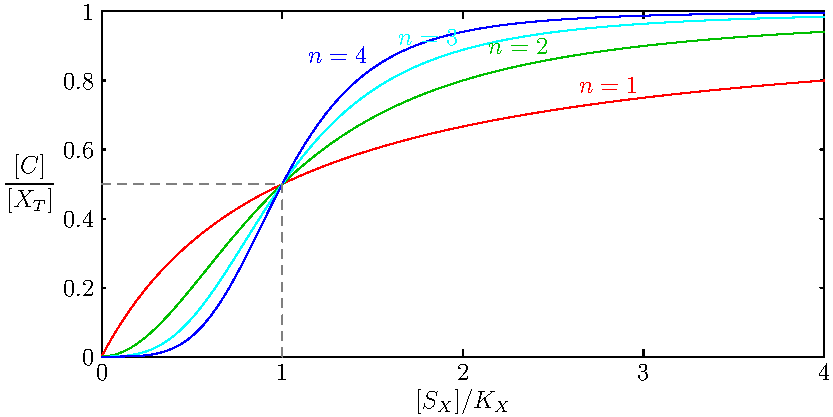
\includegraphics[width=0.62\textwidth]{./figures/hillCurves-4.pdf}
\caption{Hill Curves for differnt values of \(n\) \label{fig:hill}}
\end{figure}
\item Note that by using \(n>1\) we get a much faster switching in the
concentration of \(C\)
\item When the protein acts as a transcription factor that increases
the expression of another protein (a, so called, \emph{activator}),
then the effective rate of producing the new protein is
\[ f([S_X]) = \frac{\beta\,[X]^n}{K^n + [S_X]^n} \]
\item When \(X\) inhibits the expression of another protein (a, so
called, \emph{repressor}) then the rate of production of the other
protein is
\[ f([S_X]) = \frac{\beta}{1 + ([S_X]/K)^n} \]
\begin{figure}[htbp]
\centering
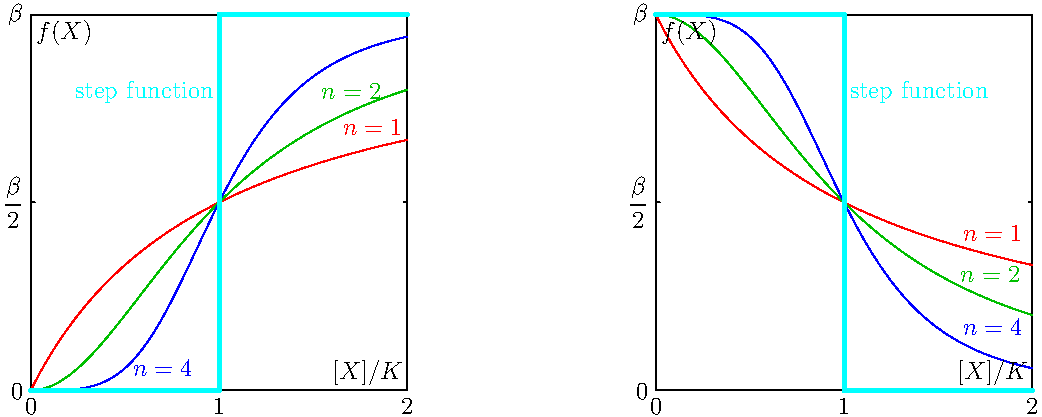
\includegraphics[width=0.7\textwidth]{./figures/activerepress.pdf}
\caption{Activator and Repressor \label{fig:activerepress}}
\end{figure}
\end{itemize}
\end{itemize}

\subsection{Motifs}
\label{sec:orgf00b775}
\begin{itemize}
\item Trying to make sense of a huge network of interacting proteins is
a real challenge
\item One common approach is to look at small sub-networks that occur
more often than we would expect by chance
\item These are called \textbf{motifs}
\item Many motifs have been studied, we will consider one example: \emph{negative auto-regulation}
\end{itemize}

\subsubsection{Auto-regulation}
\label{sec:orgf5c0fd5}
\begin{itemize}
\item When you look at gene regulation networks (GRN) there are a lot
of genes that regulate (suppress) there own production
\item To see whether this happens by chance lets look at \emph{E-coli} (one
of the most studied organisms on the planet)
\begin{itemize}
\item In \emph{E-coli} there are \(N=424\) proteins with \(E=519\) known interactions
between the proteins
\item 40 of these interactions are self-interactions
\item Could this happen by chance?
\item To calculate this we consider all possible pairwise interactions
\begin{itemize}
\item There are \(N^2\) such interactions of which \(N\) are self-interactions
\item The probability that a randomly chosen interaction is a
self-interaction is \(p=N/N^{2}=1/N\)
\item The probability that if we choose \(E\) interactions at random
\(k\) of them will be self-interactions is
\[  \Prob{k|E,p} = \mathrm{Binom}(k|E,p) =
         \binom{E}{k}\,p^k\,(1-p)^{E-k} \]
\item In expectation the number of self interactions we would expect
if they were just random was \(E\,p \approx 1.2\) with a
standard deviation of \(\sigma = \sqrt{E\,p\,(1-p)}\approx 1.1\)
\item As we have 40 self-interactions this is \(32\,\sigma\) above
the mean, which isn't going to happen by chance!
\end{itemize}
\end{itemize}
\item So what do self-interaction do?
\item Most of these self-interactions are inhibitory
\item To understand this we can model the production of a protein with
and without auto-regulation
\begin{enumerate}
\item \emph{No auto-regulation}
\begin{itemize}
\item Let's start with a protein, \(\hat{X}\), that is produce at
some rate, \(\hat{\alpha}\) and decays at a rate \(\hat{\beta}\)
\[ \varnothing \stackrel{\hat{\beta}}{\longrightarrow} \hat{X} \qquad
           \hat{X} \stackrel{\hat{\alpha}}{\longrightarrow}
          \varnothing \]
\item The ODE for this process is
\[ \frac{\dd [\hat{X}]}{\dd t} = \hat{\beta} -
          \hat{\alpha}\, [\hat{X}] \]
\item At steady state \(\hat{[X]} = \hat{\beta}/\hat{\alpha}\)
\item This is a linear ODE we can actually solve in closed form
(assuming \([\hat{X}(0)]=0\))
\[ [\hat{X}(t)] = \frac{\hat{\beta}}{\hat{\alpha}}
                      \left( 1- \e{-\hat{\alpha}\,t} \right) \]
\end{itemize}
\item \emph{Auto-regulation}
\begin{itemize}
\item We assume that a protein \(X\) acts a repressor for itself
\[ \frac{\dd [X]}{\dd t} = f([X]) - \alpha \, [X] \]
\item \(f([X])\) is a Hill repressor
\[ f([X]) = \frac{\beta}{1 + ([X]/K)^n} \approx
          \beta\,\pred{[X]<K} \]
\item This is a non-linear equation which we can't solve in closed form
\item We can easily solve it numerically
\item We show the dynamics for different \(n\) when we use
\(\hat{\beta}=2\beta\)  below
\hspace*{-3cm} \begin{center}
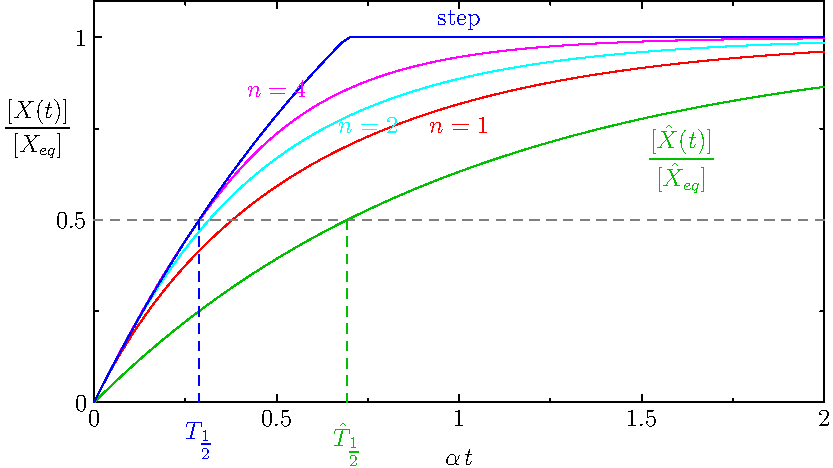
\includegraphics[width=0.55\textwidth]{./figures/autoReg.pdf}
\end{center}
\item To compare to the case without auto-regression we scale
everything so they have the same steady state
\item We also show the dynamics without auto-regression (green
line). Note that this is much slower
\item The blue line is when we replace the Hill repressor with the
step function
\item This case is solvable
\begin{itemize}
\item The dynamics is the same as the linear dynamics when
\([X]<K\) except we now produce \(X\) at a rate \(\beta = 2\,\hat{\beta}\)
\item When we reach \([X]=K\) the step switch off the production
of \(X\)
\item The steady state in this case is determined by \(K\) (as
opposed to \(\hat{\beta}\) when we have no auto-regulation)
\item We can make this reaction as fast as we like by increasing \(\beta\)
\item This isn't possible for the case without auto-regulation
because when we increase \(\beta\) we change the steady
state and our time to reach the steady state is just the same
\end{itemize}
\item Thus the advantage of negative auto-regulation is that we can speed
up the time to reach the equilibrium value
\item A subtler advantage is that \(\beta\) and \(\alpha\) can
fluctuate during the life cycle of the cell (for example, as
the cell increases in size the concentration of \(\RNA_X\) may change)
\item On the other hand, for auto-regulation the value of \(K\) is
depends on the chemical bonds at the binding site for \(X\)
which is more stable
\end{itemize}
\end{enumerate}
\end{itemize}

\section{Exercises}
\label{sec:org1ab0a50}

\subsection{Chemical Equations}
\label{sec:orga6b3c71}
\begin{enumerate}
\item Write down the ODE for the following chemical equations
\begin{align*}
 2\, X + Y  &\stackrel{k_1}{\longrightarrow} Y + Z\\
 Z &\stackrel{k_2}{\longrightarrow} \varnothing
\end{align*}
\item And for
 \begin{align*}
 X  &\stackrel{k_1}{\longrightarrow} 2\,X + Z\\
 Z &\stackrel{k_2}{\longrightarrow} 3\,Y
\end{align*}
\end{enumerate}


\section{Answers}
\label{sec:orgadb3bfa}

\subsection{Chemical Equations}
\label{sec:org5272f73}
\begin{enumerate}
\item \begin{align*}
 \frac{\dd X}{\dd t} &= -2\,k_1\,[X]^2\,[Y]  &
 \frac{\dd Y}{\dd t} &= 0 &
 \frac{\dd Z}{\dd t} & = k_1\,[X]^2\,[Y]  - k_2 \, [Z]
\end{align*}
\item \begin{align*}
\frac{\dd X}{\dd t} &= k_1\, [X] &
\frac{\dd Y}{\dd t} &= 3\,k_2 \,[Z] &
\frac{\dd Z}{\dd t} &=  k_1\, [X] - k_2 \,[Z]
\end{align*}
\end{enumerate}
\end{document}
